% =====================================================================
%  From High-School Maths to HATI -- a self-contained course
%  A companion that builds every prerequisite for hati_math.pdf
%  Author: Gergő Csaba Morvai      Engine: LuaLaTeX
%  Build: latexmk -lualatex hati_textbook.tex
% =====================================================================
\documentclass[11pt,oneside]{book}

\usepackage{fontspec}
\usepackage{microtype}
\usepackage[a4paper,margin=2.4cm]{geometry}
\usepackage{amsmath,amssymb,mathtools}
\usepackage{siunitx}
\sisetup{detect-all}
\usepackage{xcolor}
\usepackage{tikz}
\usetikzlibrary{positioning,arrows.meta,calc,decorations.pathmorphing,backgrounds}
\usepackage{tcolorbox}
\tcbuselibrary{skins,breakable}
\usepackage{titlesec}
\usepackage{enumitem}
\usepackage[hidelinks]{hyperref}

\setmainfont{TeX Gyre Pagella}
\setsansfont{TeX Gyre Heros}[Scale=0.92]
\setmonofont{TeX Gyre Cursor}[Scale=0.9]

% ---- palette ----
\definecolor{ink}{HTML}{1F3A5F}
\definecolor{warm}{HTML}{B9651F}
\definecolor{grn}{HTML}{1B7A6E}
\definecolor{blu}{HTML}{2E6DB4}
\definecolor{pur}{HTML}{6A4CA0}
\definecolor{red}{HTML}{B23A2E}
\definecolor{tealx}{HTML}{0E7C86}

% ---- chapter / section styling ----
\titleformat{\chapter}[display]
  {\sffamily\bfseries\color{ink}}
  {\filright\Large\color{ink!70}Chapter \thechapter}
  {0.4ex}{\Huge}
\titlespacing*{\chapter}{0pt}{6pt}{18pt}
\titleformat{\section}{\sffamily\large\bfseries\color{ink}}{\thesection}{0.6em}{}
\titleformat{\subsection}{\sffamily\normalsize\bfseries\color{ink!85}}{\thesubsection}{0.5em}{}

% ---- pedagogical boxes ----
\newtcolorbox{intuition}{breakable,enhanced,colback=warm!7,colframe=warm,boxrule=0.6pt,
  arc=2pt,left=7pt,right=7pt,top=4pt,bottom=4pt,fonttitle=\bfseries\sffamily\small,
  coltitle=warm,attach boxed title to top left={xshift=8pt,yshift=-7pt},
  boxed title style={colback=warm!7,colframe=warm,boxrule=0.4pt,arc=1pt},title={Intuition first}}
\newtcolorbox{keyidea}{breakable,enhanced,colback=grn!8,colframe=grn,boxrule=0.6pt,
  arc=2pt,left=7pt,right=7pt,top=4pt,bottom=4pt,fonttitle=\bfseries\sffamily\small,
  coltitle=grn,attach boxed title to top left={xshift=8pt,yshift=-7pt},
  boxed title style={colback=grn!8,colframe=grn,boxrule=0.4pt,arc=1pt},title={The key idea}}
\newtcolorbox{example}{breakable,enhanced,colback=blu!7,colframe=blu,boxrule=0.6pt,
  arc=2pt,left=7pt,right=7pt,top=4pt,bottom=4pt,fonttitle=\bfseries\sffamily\small,
  coltitle=blu,attach boxed title to top left={xshift=8pt,yshift=-7pt},
  boxed title style={colback=blu!7,colframe=blu,boxrule=0.4pt,arc=1pt},title={Worked example}}
\newtcolorbox{hatibox}{breakable,enhanced,colback=pur!7,colframe=pur,boxrule=0.6pt,
  arc=2pt,left=7pt,right=7pt,top=4pt,bottom=4pt,fonttitle=\bfseries\sffamily\small,
  coltitle=pur,attach boxed title to top left={xshift=8pt,yshift=-7pt},
  boxed title style={colback=pur!7,colframe=pur,boxrule=0.4pt,arc=1pt},title={Where this lives in HATI}}
\newtcolorbox{pitfall}{breakable,enhanced,colback=red!6,colframe=red,boxrule=0.6pt,
  arc=2pt,left=7pt,right=7pt,top=4pt,bottom=4pt,fonttitle=\bfseries\sffamily\small,
  coltitle=red,attach boxed title to top left={xshift=8pt,yshift=-7pt},
  boxed title style={colback=red!6,colframe=red,boxrule=0.4pt,arc=1pt},title={Watch out}}
\newtcolorbox{practice}{breakable,enhanced,colback=tealx!7,colframe=tealx,boxrule=0.6pt,
  arc=2pt,left=7pt,right=7pt,top=4pt,bottom=4pt,fonttitle=\bfseries\sffamily\small,
  coltitle=tealx,attach boxed title to top left={xshift=8pt,yshift=-7pt},
  boxed title style={colback=tealx!7,colframe=tealx,boxrule=0.4pt,arc=1pt},title={Practice}}
\newtcolorbox{defn}{breakable,enhanced,colback=ink!5,colframe=ink!60,boxrule=0.6pt,
  arc=2pt,left=7pt,right=7pt,top=4pt,bottom=4pt,fonttitle=\bfseries\sffamily\small,
  coltitle=ink,attach boxed title to top left={xshift=8pt,yshift=-7pt},
  boxed title style={colback=ink!5,colframe=ink!60,boxrule=0.4pt,arc=1pt},title={Definition}}

\newcommand{\norm}[1]{\left\lVert #1\right\rVert}
\newcommand{\abs}[1]{\left\lvert #1\right\rvert}
\newcommand{\R}{\mathbb{R}}
\newcommand{\half}{\tfrac12}

\title{\sffamily\bfseries\color{ink}\Huge From High-School Maths to \textsc{Hati}\\[6pt]
\LARGE\mdseries A self-contained course in the mathematics of\\ lunar terrain-hazard detection}
\author{\Large Gerg\H{o} Csaba Morvai}
\date{\today}

\begin{document}
\frontmatter
\maketitle

\thispagestyle{empty}
\noindent\begin{center}\itshape
For anyone who can solve a quadratic and wants to read this and mean it:
\end{center}
\begin{equation*}
H(x)=\sigma\!\left(b+\frac{1}{\norm{\mathbf w}_1}\sum_{k=1}^{10} w_k\,
\operatorname{clip}_{\pm c}\!\left[\frac{g(C_k[z])(x)-\operatorname{med}\,g(C_k[z])}{\operatorname{IQR}\,g(C_k[z])/1.349}\right]\right).
\end{equation*}
\begin{center}\itshape
By the last page this will not look like noise. It will look like a sentence.\end{center}

\tableofcontents

% =====================================================================
\chapter*{Start here}
\addcontentsline{toc}{chapter}{Start here}
\markboth{Start here}{Start here}

The equation on the page before this one is the whole of \textsc{Hati}'s elevation
pipeline. Right now it is probably a wall of symbols. That is fine. The job of this
book is to take you, one idea at a time, from ordinary high-school maths to the point
where you can read that line aloud and explain every piece of it to someone else.

\textsc{Hati} is a tool that looks at a map of the Moon and decides where a lander
should not touch down. It does that with two kinds of mathematics: the geometry and
calculus of a bumpy surface, and the statistics and machine learning that turn
``bumpy'' into a single number between 0 and 1. Both are within your reach. Neither
requires anything you could not have met by the end of school; it just requires that
we build the ideas in the right order and never skip the meaning.

\begin{intuition}
Think of the master equation as a recipe written in shorthand. A chef reading
``fold in the egg whites'' sees a whole technique in four words. By the end of this
book each clump of symbols will be like that for you: a technique you recognise on
sight. We are going to learn the techniques first, then come back and read the recipe.
\end{intuition}

\paragraph{An honest word.} Reading this book will give you genuine understanding.
It will not, by itself, make you an expert. Nobody became fluent in a language by
reading a grammar. Expertise comes from the \textsc{Practice} boxes --- do them, with
a pen, before looking at the solutions in Appendix~B. The maths only becomes yours
when your own hand has produced it.

\paragraph{What you need before page one.} Comfort with: algebra (rearranging
$y=mx+c$), basic functions and graphs, right-angled trigonometry ($\sin,\cos,\tan$),
and the idea of a square root and a power. That is all. Everything past that --- the
calculus, the statistics, the linear algebra, the machine learning --- we build here.

\paragraph{How the book is built.} Six parts. Parts I--III build the language and the
tools. Part IV is the machine learning. Part V is the geometry and signal theory.
Part VI returns to the master equation and reads it, symbol by symbol. Every chapter
ends with a purple box, \emph{Where this lives in \textsc{Hati}}, tying the idea back
to the real pipeline, so you never learn anything without knowing why.

\mainmatter

% #####################################################################
\part{The language of the machine}

% =====================================================================
\chapter{Functions, graphs, and three special curves}

A \emph{function} is a machine: a number goes in, a number comes out, and the same
input always gives the same output. We write $f(x)$ for ``the output when the input is
$x$.'' Three particular functions run through all of \textsc{Hati}, so we meet them now.

\section{The straight line, and what a weighted sum is}
The line $f(x)=mx+c$ you already know: $m$ is the slope (how fast output climbs as
input grows), $c$ the starting height. Now stretch the idea. Suppose the output
depends on \emph{several} inputs $x_1,\dots,x_n$, each with its own importance $w_k$:
\begin{equation}
f(x_1,\dots,x_n)=w_1x_1+w_2x_2+\dots+w_nx_n + b
=\sum_{k=1}^{n}w_k x_k + b .
\end{equation}
That big-$\Sigma$ is just ``add these up''; $\sum_{k=1}^{n}a_k$ means
$a_1+a_2+\dots+a_n$. A \emph{weighted sum} is the single most important shape in this
whole book: each input gets multiplied by how much it matters, and the results are
added. Hold onto it.

\section{The exponential and the logarithm}
The exponential $e^{x}$ is the function that grows in proportion to how big it already
is (interest on interest). Its number $e\approx2.718$ is just the natural base for
that kind of growth. Two facts we will use:
\begin{equation}
e^{0}=1,\qquad e^{x}\ \text{is always positive},\qquad e^{x}\to 0 \text{ as } x\to-\infty .
\end{equation}
The logarithm $\log$ is its exact reverse: $\log(e^{x})=x$. It turns multiplication
into addition and, for us, it \emph{tames} numbers with a huge range, squashing a long
tail down to something manageable. We will use $\log(1+x)$ specifically, because it
behaves at $x=0$ (giving $0$, not $-\infty$).

\section{The logistic curve: the S that makes a decision}
Now the star. Define
\begin{equation}
\boxed{\ \sigma(a)=\frac{1}{1+e^{-a}}\ }\qquad\text{(the \emph{logistic} or \emph{sigmoid}).}
\label{eq:sigmoid}
\end{equation}
Feed it any number on the line, $-\infty$ to $+\infty$, and it answers with a number
strictly between $0$ and $1$. Check the ends: if $a$ is very negative, $e^{-a}$ is
huge, so $\sigma\to0$; if $a$ is very positive, $e^{-a}\to0$, so $\sigma\to1$; and
$\sigma(0)=\tfrac12$. It is a smooth switch.

\begin{center}
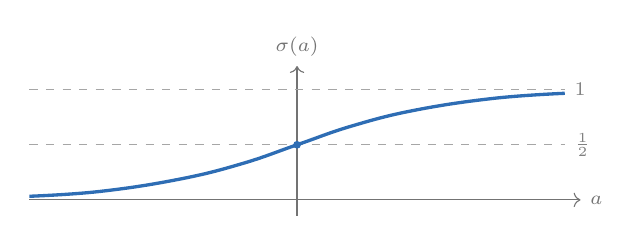
\begin{tikzpicture}[scale=1.0]
  \draw[->,black!55] (-3.4,0)--(3.6,0) node[right,font=\scriptsize]{$a$};
  \draw[->,black!55] (0,-0.2)--(0,1.7) node[above,font=\scriptsize]{$\sigma(a)$};
  \draw[dashed,black!35] (-3.4,1.4)--(3.4,1.4) node[right,font=\scriptsize,black!50]{$1$};
  \draw[dashed,black!35] (-3.4,0.7)--(3.4,0.7) node[right,font=\scriptsize,black!50]{$\tfrac12$};
  \draw[very thick,blu] plot[smooth,tension=0.7] coordinates{
    (-3.4,0.046)(-2.5,0.108)(-1.5,0.262)(-0.7,0.46)(0,0.7)(0.7,0.94)(1.5,1.14)(2.5,1.29)(3.4,1.354)};
  \fill[blu] (0,0.7) circle (1.4pt);
\end{tikzpicture}
\end{center}
(The curve is drawn with the output axis stretched so the flat-to-1 part is visible;
the shape is the point.)

\begin{keyidea}
A weighted sum produces a single number $a$ that can be anything. The sigmoid
$\sigma(a)$ then bends that number into a probability between $0$ and $1$. ``Weighted
sum, then sigmoid'' is the entire skeleton of \textsc{Hati}'s decision --- and, as
we will see in Part~IV, of the simplest machine-learning classifier ever built.
\end{keyidea}

\begin{hatibox}
In the master equation, the outermost symbol is $\sigma(\cdots)$: the very last thing
\textsc{Hati} does is squash a weighted sum through this S-curve to get the hazard
probability $H(x)$. The $g=\log(1+\cdot)$ inside it is the tail-taming log you just
met. You already recognise two pieces of the wall.
\end{hatibox}

\begin{practice}
\textbf{1.1} Compute $\sigma(0)$, and argue without a calculator whether $\sigma(2)$
is closer to $0$ or to $1$. \quad\textbf{1.2} A weighted sum has weights $w=(2,-1)$,
bias $b=-1$, inputs $x=(1.5,1)$. Find $a=\sum w_kx_k+b$, then $\sigma(a)$ (a calculator
is fine). \quad\textbf{1.3} Why would $\log(x)$ be a bad ``tail-tamer'' for a quantity
that can equal $0$, and why does $\log(1+x)$ fix it?
\end{practice}

% =====================================================================
\chapter{The trigonometry you will actually use}

You met $\sin,\cos,\tan$ as ratios of sides in a right triangle. \textsc{Hati} uses
exactly two ideas from that: turning a ratio into an angle, and turning an angle into
a length.

\section{Slope is an angle}
Walk one metre east and rise $r$ metres. The steepness is the ratio $r/1=r$ (``rise
over run''), but it is often nicer as an \emph{angle} $\theta$ above horizontal, and
the two are linked by the tangent:
\begin{equation}
\tan\theta=\frac{\text{rise}}{\text{run}}\quad\Longleftrightarrow\quad
\theta=\arctan\!\left(\frac{\text{rise}}{\text{run}}\right).
\end{equation}
$\arctan$ (``inverse tangent'') is just the button that turns a ratio back into the
angle that produced it. A flat surface has $\theta=0$; a $45^\circ$ slope has
$\tan\theta=1$.

\section{A shadow is a ruler}
Here is the other side of the same triangle. The Sun sits at an angle $e$ above the
horizon. An object of height $h$ casts a shadow of length $L$ on flat ground. The Sun
ray grazes the top of the object and hits the ground at the shadow's tip, making a
right triangle with the object (height $h$) and the shadow (length $L$):
\begin{equation}
\tan e=\frac{h}{L}\qquad\Longrightarrow\qquad \boxed{\,h=L\tan e.\,}
\label{eq:shadow}
\end{equation}

\begin{center}
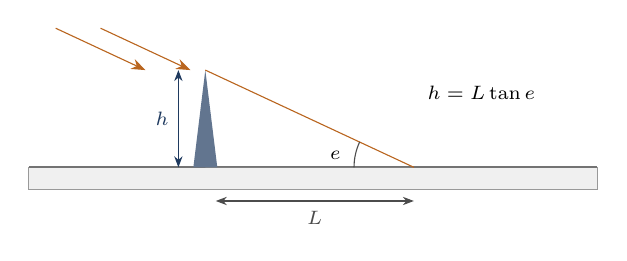
\begin{tikzpicture}[scale=0.95]
  \draw[fill=black!6,draw=black!40] (-0.2,0) rectangle (7.4,-0.3);
  \draw[thick,black!55] (-0.2,0)--(7.4,0);
  \def\hh{1.3}\pgfmathsetmacro{\LL}{\hh/tan(25)}
  \fill[ink!70] (2,0)--(2.16,\hh)--(2.32,0)--cycle;
  \coordinate(T) at (2.16,\hh);\coordinate(S) at ({2.16+\LL},0);
  \fill[black!20] (2.32,0)--(S)--(2.16,0)--cycle;
  \foreach \dx in {-0.8,-0.2}{\draw[-{Stealth[length=1.8mm]},warm]
     ($(T)+(\dx,0)+(-1.2,{1.2*tan(25)})$)--($(T)+(\dx,0)$);}
  \draw[warm] (T)--(S);
  \draw[black!70] (S)++(-0.8,0) arc (180:155:0.8); \node[font=\scriptsize] at ($(S)+(-1.05,0.16)$){$e$};
  \draw[{Stealth[length=1.4mm]}-{Stealth[length=1.4mm]},ink](1.8,0)--(1.8,\hh) node[midway,left,font=\scriptsize]{$h$};
  \draw[{Stealth[length=1.4mm]}-{Stealth[length=1.4mm]},black!70](2.3,-0.45)--($(S)+(0,-0.45)$) node[midway,below,font=\scriptsize]{$L$};
  \node[font=\scriptsize,anchor=west] at (5.0,1.0){$h=L\tan e$};
\end{tikzpicture}
\end{center}

The lower the Sun (small $e$), the longer the shadow for a given height --- which is
why the lunar pole, where the Sun barely clears the horizon, turns even tiny rocks
into long, measurable shadows.

\begin{hatibox}
Channel~2 of \textsc{Hati} measures shadow lengths $L$ in a photograph and uses
Equation~\eqref{eq:shadow} to recover obstacle heights $h$ --- seeing rocks far too
small for the elevation map. The slope-as-angle idea (Section~2.1) is how
\textsc{Hati} turns the steepness of the terrain into the slope field it then measures
the roughness of.
\end{hatibox}

\begin{practice}
\textbf{2.1} A boulder casts a \SI{6}{m} shadow with the Sun $20^\circ$ up. How tall
is it? \quad\textbf{2.2} The same boulder at sunset, Sun only $5^\circ$ up --- now how
long is its shadow? What does this say about the best time to hunt for small hazards?
\end{practice}

% =====================================================================
\chapter{Vectors and the dot product}

\textsc{Hati} describes each spot on the Moon by ten numbers at once. To handle ``ten
numbers as one object'' we need vectors.

\begin{defn}
A \emph{vector} is an ordered list of numbers, written
$\mathbf v=(v_1,v_2,\dots,v_n)$. The number $n$ is its \emph{dimension}. A point on a
map is a 2-vector $(X,Y)$; a spot described by ten roughness numbers is a 10-vector.
\end{defn}

\section{The dot product is a weighted sum in disguise}
Given two vectors of the same length, their \emph{dot product} multiplies matching
entries and adds:
\begin{equation}
\mathbf w\cdot\mathbf x=\mathbf w^{\mathsf T}\mathbf x=\sum_{k=1}^{n}w_kx_k
= w_1x_1+\dots+w_nx_n .
\end{equation}
Look familiar? It is exactly the weighted sum from Chapter~1. So if $\mathbf x$ holds
the ten roughness numbers for a spot and $\mathbf w$ holds how much each one matters,
then $\mathbf w\cdot\mathbf x$ is ``the overall hazard vote'' in a single product.

\begin{intuition}
A vector is a labelled bag of numbers you can carry around as one thing. The dot
product asks: ``how much do these two bags agree, weighted entry by entry?'' Big
positive dot product means the inputs that matter most are large. That is precisely
the score we want to feed the sigmoid.
\end{intuition}

\begin{hatibox}
The fraction $\frac{1}{\norm{\mathbf w}_1}\mathbf w^{\mathsf T}\boldsymbol\zeta$ inside
the master equation is a dot product: $\boldsymbol\zeta$ is the vector of ten
standardised roughness numbers, $\mathbf w$ the literature weights, and
$\norm{\mathbf w}_1=\sum_k\abs{w_k}$ is a scaling so the result does not balloon as we
add channels. The whole of Chapter~7 in \texttt{hati\_math.pdf} is built on this one
product.
\end{hatibox}

\begin{practice}
\textbf{3.1} With $\mathbf w=(1,0.7,0.7)$ and $\mathbf x=(2,-1,3)$, compute
$\mathbf w\cdot\mathbf x$. \quad\textbf{3.2} If every weight is positive and one input
doubles while the rest stay fixed, can the dot product go down? What does that tell you
about how a single rough channel affects \textsc{Hati}'s vote?
\end{practice}

% #####################################################################
\part{Calculus on a grid}

% =====================================================================
\chapter{Derivatives and the gradient}

\section{The derivative: instantaneous steepness}
Zoom in on the graph of $f(x)$ until the curve looks straight. The slope of that tiny
straight piece is the \emph{derivative} $f'(x)$, written also $\dfrac{df}{dx}$. It is
the rate of change: how fast the output moves when you nudge the input. Formally it is
the limit of rise-over-run as the run shrinks to nothing,
\begin{equation}
f'(x)=\lim_{\Delta x\to0}\frac{f(x+\Delta x)-f(x)}{\Delta x},
\end{equation}
but the picture --- ``slope of the curve right here'' --- is what you need.

\begin{example}
For $f(x)=x^2$, nudging from $x$ to $x+\Delta x$ changes the output by
$(x+\Delta x)^2-x^2=2x\Delta x+\Delta x^2$. Divide by $\Delta x$: $2x+\Delta x$. As
$\Delta x\to0$ this is $2x$. So $f'(x)=2x$: at $x=3$ the curve rises three-to-one
steeper than at $x=1$. We just did calculus from scratch.
\end{example}

\section{Many inputs: partial derivatives and the gradient}
Terrain height depends on two inputs: position east ($X$) and north ($Y$). The
\emph{partial derivative} $\partial z/\partial X$ is the slope you feel walking purely
east (holding $Y$ fixed); $\partial z/\partial Y$ is the slope walking purely north.
Pack the two into a vector, the \emph{gradient}:
\begin{equation}
\nabla z=\left(\frac{\partial z}{\partial X},\ \frac{\partial z}{\partial Y}\right).
\end{equation}

\begin{keyidea}
The gradient points in the direction of \emph{steepest uphill}, and its length is how
steep that is. On a hillside, $\nabla z$ is the arrow water would flow against. The
overall steepness --- the \emph{slope} --- is just the length of that arrow,
$\norm{\nabla z}=\sqrt{(\partial z/\partial X)^2+(\partial z/\partial Y)^2}$, by
Pythagoras.
\end{keyidea}

So the slope angle of the ground is
\begin{equation}
\sigma_{\text{slope}}=\arctan\norm{\nabla z}=\arctan\sqrt{(\partial_X z)^2+(\partial_Y z)^2},
\end{equation}
combining the gradient (this chapter) with arctan (Chapter~2).

\begin{hatibox}
Every roughness channel in \textsc{Hati} starts from this slope field. ``Rough''
ultimately means ``the gradient is large and changes a lot from spot to spot.'' The
gradient is the first thing the pipeline computes from the raw elevation grid.
\end{hatibox}

\begin{practice}
\textbf{4.1} Find $f'(x)$ for $f(x)=3x^2$ by the nudge method. \quad\textbf{4.2} A
patch has $\partial_X z=0.1$ and $\partial_Y z=0$ (metres per metre). What is the slope
angle? Now $\partial_X z=\partial_Y z=0.1$: is it steeper or shallower, and why does
Pythagoras say so?
\end{practice}

% =====================================================================
\chapter{Curvature and the Laplacian}

The first derivative tells you the slope; the \emph{second} derivative tells you how
the slope is changing --- whether the ground is bending into a bowl or over a dome.

For one input, the second derivative $f''(x)$ is just the derivative of $f'$. Positive
$f''$ means the slope is increasing: the curve holds water (a bowl, like $x^2$).
Negative $f''$ means a dome.

For terrain (two inputs) the natural single measure of bending adds the two
straight-line curvatures:
\begin{equation}
\nabla^2 z=\frac{\partial^2 z}{\partial X^2}+\frac{\partial^2 z}{\partial Y^2}
\qquad\text{(the \emph{Laplacian}).}
\end{equation}
It is positive in a pit (a crater floor), negative on a peak (a rim or boulder top),
and zero on anything flat or evenly tilted.

\begin{intuition}
Stand a marble on the surface. Where it would settle (a pit), the Laplacian is
positive; where it would roll off in every direction (a peak), negative; on a ramp, it
neither settles nor has a preferred runaway, so zero. The Laplacian is a one-number
``bowl-ness'' meter --- and a crater is a ring of negative rim around a positive floor,
a signature the Laplacian sees clearly.
\end{intuition}

\begin{hatibox}
\textsc{Hati}'s curvature channel measures how much the Laplacian \emph{varies} across
a small window. Smooth ground has near-constant curvature; a crater field has curvature
swinging from rim to floor. That swing is one of \textsc{Hati}'s strongest hazard
signals.
\end{hatibox}

\begin{practice}
\textbf{5.1} For $f(x)=x^2$ we found $f'(x)=2x$. What is $f''(x)$? Is it a bowl or a
dome? \quad\textbf{5.2} Sketch a cross-section of a crater (down then up) and mark
where the curvature is positive and where negative.
\end{practice}

% =====================================================================
\chapter{Pixels, finite differences, and convolution}

Real elevation data is not a smooth formula --- it is a \emph{grid of numbers}, one
height per pixel. So we need derivatives we can compute by arithmetic on neighbours.

\section{Finite differences}
The derivative is rise over run; on a grid the smallest run is one pixel. So the slope
in the $X$ direction at pixel $(i,j)$ is approximately the right neighbour minus the
left neighbour, over the distance:
\begin{equation}
\frac{\partial z}{\partial X}\approx\frac{z_{i,j+1}-z_{i,j-1}}{2s},
\end{equation}
where $s$ is the pixel size in metres. Curvature uses ``neighbour $+$ neighbour $-$
twice the centre,'' which on a grid becomes the five-point pattern
$z_{i,j+1}+z_{i,j-1}+z_{i+1,j}+z_{i-1,j}-4z_{i,j}$.

\section{Convolution: sliding a little stencil}
Doing the same little weighted combination of neighbours at \emph{every} pixel has a
name: \emph{convolution}. You take a small grid of weights --- a \emph{kernel} --- lay
it over each pixel, multiply overlapping numbers, and add. The Sobel kernel for the
east--west slope and the Laplacian kernel for curvature are
\begin{equation}
K_x=\begin{pmatrix}-1&0&1\\-2&0&2\\-1&0&1\end{pmatrix},\qquad
K_L=\begin{pmatrix}0&1&0\\1&-4&1\\0&1&0\end{pmatrix}.
\end{equation}

\begin{center}
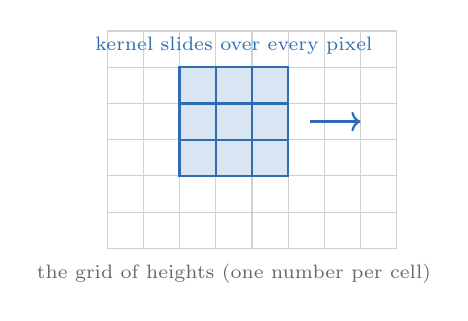
\begin{tikzpicture}[scale=0.46]
  \foreach \x in {0,...,7}\foreach \y in {0,...,5}{\draw[black!18](\x,\y) rectangle (\x+1,\y+1);}
  \fill[blu!18] (2,2) rectangle (5,5);
  \foreach \x in {2,3,4}\foreach \y in {2,3,4}{\draw[blu,thick](\x,\y) rectangle (\x+1,\y+1);}
  \node[blu,font=\scriptsize] at (3.5,5.6){kernel slides over every pixel};
  \draw[->,blu,thick] (5.6,3.5)--(7.0,3.5);
  \node[font=\scriptsize,black!60] at (3.5,-0.7){the grid of heights (one number per cell)};
\end{tikzpicture}
\end{center}

\begin{keyidea}
A convolution is just ``do the same small neighbour-recipe at every pixel.'' Slopes,
curvature, and even blurring are all convolutions with different little kernels. It is
the workhorse that turns a static grid of heights into fields of slope and curvature.
\end{keyidea}

\begin{hatibox}
The symbols $C_k[z]$ in the master equation are these operations: each channel is a
convolution (or a close cousin) applied to the elevation grid $z$. The kernels above
are literally the first lines of \textsc{Hati}'s code.
\end{hatibox}

\begin{practice}
\textbf{6.1} A row of heights is $\dots,4,4,4,9,4,4,\dots$ (one tall pixel). Apply the
1-D curvature recipe ``left $+$ right $-2\times$centre'' at the $9$. Is the result
positive or negative, and does that match ``a bump''? \quad\textbf{6.2} What does a
kernel of all $\tfrac19$'s (a $3\times3$ of ninths) do to an image? (Hint: it is an
average.)
\end{practice}

% #####################################################################
\part{Reading the data}

% =====================================================================
\chapter{Describing a pile of numbers}

A window of the slope field is just a pile of numbers. We need to summarise it.

\begin{defn}
For values $x_1,\dots,x_n$: the \emph{mean} is $\bar x=\frac1n\sum x_k$ (the balance
point). The \emph{variance} is $\frac1n\sum(x_k-\bar x)^2$ (average squared distance
from the mean); its square root is the \emph{standard deviation}, the typical spread.
The \emph{root-mean-square} (RMS) is $\sqrt{\frac1n\sum x_k^2}$ --- the typical size,
ignoring sign.
\end{defn}

Those are \emph{moment} summaries: they add things up. There is a second family that
\emph{sorts} instead. Line the values up smallest to largest. The \emph{median} is the
middle one. The value with a quarter of the data below it is the lower quartile
$Q_{25}$; three-quarters below, the upper quartile $Q_{75}$. Their gap is the
\emph{interquartile range},
\begin{equation}
\operatorname{IQR}=Q_{75}-Q_{25},
\end{equation}
a measure of spread that uses position, not arithmetic.

\begin{intuition}
Mean and RMS \emph{compute}; median and IQR \emph{rank}. The difference matters because
one wild value can drag a mean a long way but barely budges a median. We will lean on
that robustness in the next chapter.
\end{intuition}

\begin{hatibox}
\textsc{Hati}'s ten channels are exactly these summaries applied to slope and curvature
inside a sliding window: RMS of slope, IQR of slope, IQR of curvature, and so on. ``How
rough is this patch'' is answered by ``how spread out are its slopes,'' and spread is
mean-square or IQR.
\end{hatibox}

\begin{practice}
\textbf{7.1} Find the mean and the median of $\{1,2,2,3,40\}$. Which one ``feels'' like
the typical value, and why is the other misleading? \quad\textbf{7.2} For
$\{1,2,3,4,5,6,7,8\}$ find $Q_{25}$, $Q_{75}$, and the IQR.
\end{practice}

% =====================================================================
\chapter{The bell curve and robust statistics}

\section{The normal distribution}
Measure many natural things and their histogram piles up in the famous symmetric
``bell'': most values near a central one, fewer as you go out, tails thinning fast.
This is the \emph{normal} (or Gaussian) distribution, with a centre $\mu$ and a spread
$s$. Its great convenience: fixed fractions of the data sit within fixed multiples of
$s$ from the centre, always.

\begin{center}
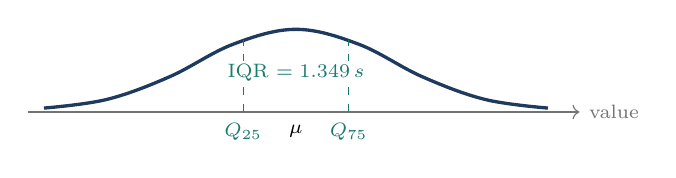
\begin{tikzpicture}[scale=1.0]
  \draw[->,black!55] (-3.4,0)--(3.6,0) node[right,font=\scriptsize]{value};
  \draw[very thick,ink] plot[smooth,tension=0.6] coordinates{
    (-3.2,0.05)(-2.4,0.16)(-1.6,0.45)(-0.8,0.86)(0,1.05)(0.8,0.86)(1.6,0.45)(2.4,0.16)(3.2,0.05)};
  \draw[dashed,grn] (-0.67,0)--(-0.67,0.92); \draw[dashed,grn] (0.67,0)--(0.67,0.92);
  \node[grn,font=\scriptsize] at (-0.67,-0.25){$Q_{25}$}; \node[grn,font=\scriptsize] at (0.67,-0.25){$Q_{75}$};
  \draw[<->,grn] (-0.67,0.5)--(0.67,0.5); \node[grn,font=\scriptsize,fill=white,inner sep=1pt] at (0,0.5){IQR $=1.349\,s$};
  \node[font=\scriptsize] at (0,-0.25){$\mu$};
\end{tikzpicture}
\end{center}

\section{Why median and IQR, and where 1.349 comes from}
Mean and standard deviation are easy prey for outliers: a single huge value inflates
both. Median and IQR shrug it off, because moving one extreme value does not move the
middle or the quartiles. Statisticians call methods with this property \emph{robust}.

But the IQR is on a different scale from the standard deviation. For a normal curve the
quartiles sit at $\pm0.6745\,s$ from the centre (that $0.6745$ is just where the bell
cuts off a quarter of its area). So
\begin{equation}
\operatorname{IQR}=0.6745\,s-(-0.6745\,s)=1.349\,s
\quad\Longrightarrow\quad
\hat s=\frac{\operatorname{IQR}}{1.349}.
\end{equation}
Dividing the IQR by $1.349$ converts a robust spread back into ordinary
standard-deviation units. That mysterious constant in the master equation is nothing
but the width of a bell curve measured in IQRs.

\begin{pitfall}
$1.349$ is \emph{not} a tuning knob someone fiddled. It is forced by the geometry of
the normal curve. If you ever see it and think ``magic number,'' remember: it is
$2\times0.6745$, and $0.6745$ is the quartile of the standard bell.
\end{pitfall}

\begin{hatibox}
The denominator $\operatorname{IQR}\,g(C_k[z])/1.349$ in the master equation is this
exact conversion, applied to each channel: it measures each roughness field's spread
robustly, then rescales it to standard-deviation units so all ten channels speak the
same language.
\end{hatibox}

\begin{practice}
\textbf{8.1} A channel has $\operatorname{IQR}=2.698$. Estimate its standard deviation.
\quad\textbf{8.2} Add the value $1000$ to the set $\{1,2,3,4,5\}$. By how much does the
median move? The mean? Which is robust?
\end{practice}

% =====================================================================
\chapter{Standardizing features}

Ten channels in ten different units cannot be compared, let alone added. We put them on
one ruler in three steps, all visible in the master equation.

\begin{enumerate}[leftmargin=1.4em]
\item \textbf{Tame the tail:} apply $g(x)=\log(1+x)$. Roughness values have a few huge
outliers; the log squashes them without changing their order.
\item \textbf{Centre and scale (the $z$-score):} subtract the median, divide by
$\operatorname{IQR}/1.349$:
\[
\zeta=\frac{g(C)-\operatorname{med}\,g(C)}{\operatorname{IQR}\,g(C)/1.349}.
\]
Now $\zeta$ is in ``spreads from typical'': $\zeta=+2$ means ``two spreads rougher than
normal,'' and it means the same thing in every channel.
\item \textbf{Clip:} cap $\zeta$ at $\pm4$ so no single freak pixel can dominate.
\end{enumerate}

\begin{keyidea}
\emph{Standardising} strips away units and scale so different measurements become
comparable. After it, ``$+2$'' is rough in every channel alike, and adding them up
(the weighted sum) finally makes sense.
\end{keyidea}

\section{Ranking a result: percentiles}
Once we have a hazard score for every pixel, we ask of one spot: \emph{what fraction of
the map is less hazardous than this?} That fraction is its \emph{percentile}. The
function that returns it --- ``share of values at or below $t$'' --- is the
\emph{empirical cumulative distribution}. The Athena touchdown landed at the
$96$th percentile: rougher than $96\%$ of the site.

\begin{hatibox}
The big bracketed fraction inside the master equation, log on top, IQR/1.349 on the
bottom, with a $\operatorname{clip}_{\pm c}$ around it, is exactly this standardisation
done to each $C_k$. You can now read the entire inside of the sum.
\end{hatibox}

\begin{practice}
\textbf{9.1} A channel value gives $g(C)=3.0$; the field has median $1.0$ and
$\operatorname{IQR}=1.349$. Find $\zeta$. \quad\textbf{9.2} If a score beats $19$ of the
other $19$ pixels in a $20$-pixel scene, what percentile is it?
\end{practice}

% #####################################################################
\part{The machine learning}

% =====================================================================
\chapter{Probability in one bite}

A \emph{probability} is a number from $0$ to $1$ measuring how likely something is. We
need only the simplest case: a yes/no outcome (\emph{Bernoulli}). Label a site $y=1$ if
hazardous, $y=0$ if safe. A model that outputs $H\in(0,1)$ is claiming
``$\Pr(\text{hazard})=H$.''

If the truth is $y=1$ and the model said $H$, it assigned probability $H$ to what
happened; if $y=0$, it assigned $1-H$. A compact way to write ``the probability the
model gave to the actual outcome'' is
\begin{equation}
H^{\,y}(1-H)^{\,1-y},
\end{equation}
which equals $H$ when $y=1$ and $1-H$ when $y=0$ (anything to the power $0$ is $1$).
This little expression is the seed of all the learning in the next chapter.

\begin{intuition}
A good model gives high probability to things that actually happen. So if we collect
the probabilities it assigned to every real outcome and multiply them, a better model
makes that product bigger. ``Make the product of assigned probabilities as large as
possible'' is, almost word for word, how machines learn.
\end{intuition}

\begin{practice}
\textbf{10.1} A model says $H=0.8$. Write the value of $H^y(1-H)^{1-y}$ for the case
$y=1$ and for $y=0$. Which outcome was it more confident about?
\end{practice}

% =====================================================================
\chapter{The logistic neuron}

Now we assemble Parts I--III into the simplest machine-learning classifier, and
discover it \emph{is} \textsc{Hati}'s fusion step.

Take the feature vector $\boldsymbol\zeta$ (the standardised channels), dot it with
weights $\mathbf w$, add a bias $b$, and squash with the sigmoid:
\begin{equation}
H=\sigma(\mathbf w\cdot\boldsymbol\zeta+b).
\label{eq:neuron}
\end{equation}
That is a \emph{logistic-regression unit}, also called a single \emph{neuron}. The
weighted sum scores the evidence; the sigmoid turns the score into a probability.

\begin{center}
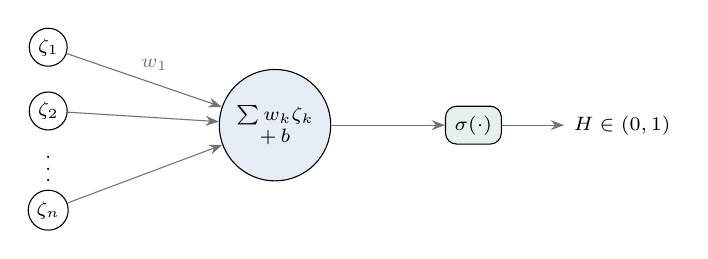
\begin{tikzpicture}[scale=0.9,>=Stealth]
  \node[draw,circle,inner sep=1.4pt,font=\scriptsize] (i1) at (0,1.5){$\zeta_1$};
  \node[draw,circle,inner sep=1.4pt,font=\scriptsize] (i2) at (0,0.6){$\zeta_2$};
  \node[font=\scriptsize] at (0,-0.1){$\vdots$};
  \node[draw,circle,inner sep=1.4pt,font=\scriptsize] (i3) at (0,-0.8){$\zeta_n$};
  \node[draw,circle,fill=blu!12,minimum size=12mm,font=\scriptsize,align=center] (S) at (3.2,0.4){$\sum w_k\zeta_k$\\$+\,b$};
  \node[draw,rounded corners,fill=grn!12,font=\scriptsize] (sig) at (6.0,0.4){$\sigma(\cdot)$};
  \node[font=\scriptsize] (out) at (8.1,0.4){$H\in(0,1)$};
  \draw[->,black!55] (i1)--(S); \draw[->,black!55] (i2)--(S); \draw[->,black!55] (i3)--(S);
  \draw[->,black!55] (S)--(sig); \draw[->,black!55] (sig)--(out);
  \node[font=\scriptsize,black!55] at (1.5,1.25){$w_1$};
\end{tikzpicture}
\end{center}

\begin{keyidea}
``Weighted sum, then sigmoid'' --- the skeleton from Chapter~1 --- is a complete
classifier. Stack many of these neurons and you have a neural network; the only new
idea is how to \emph{choose} the weights, which is the next chapter.
\end{keyidea}

\begin{hatibox}
Equation~\eqref{eq:neuron} \emph{is} the master equation, with $\mathbf w\cdot\boldsymbol
\zeta$ written as the dot product. \textsc{Hati} differs from textbook
machine learning in one deliberate way: it does not \emph{learn} $\mathbf w$ from data;
it \emph{sets} $\mathbf w$ from physics and the published literature. That is why it
needs no training labels and why every weight has a stateable reason --- the property
that makes it trustworthy for a spacecraft.
\end{hatibox}

\begin{practice}
\textbf{11.1} With $\mathbf w=(1,1)$, $b=-1$, and $\boldsymbol\zeta=(2,0)$, find $H$.
Now $\boldsymbol\zeta=(-2,0)$. Interpret the two answers as ``hazard'' or ``safe.''
\end{practice}

% =====================================================================
\chapter{Learning the weights}

\textsc{Hati} fixes its weights. But the natural next step --- and the heart of machine
learning --- is to \emph{learn} them from examples. Here is how, end to end.

\section{A score for how wrong we are}
From Chapter~10, a good model makes the product of assigned probabilities large.
Multiplying many small numbers is awkward, so we take a logarithm (turning products
into sums) and flip the sign (so ``small is good''). The result is the
\emph{cross-entropy loss}:
\begin{equation}
J=-\frac1D\sum_{m=1}^{D}\Big[y_m\log H_m+(1-y_m)\log(1-H_m)\Big].
\end{equation}
$J$ is large when the model confidently says the wrong thing, near $0$ when it is
confidently right. Learning $=$ making $J$ small.

\section{Rolling downhill: gradient descent}
$J$ depends on the weights. Picture $J$ as a landscape and the weights as your
position; you want the valley floor. The gradient $\partial J/\partial\mathbf w$ points
uphill, so step the opposite way:
\begin{equation}
\mathbf w\leftarrow\mathbf w-\eta\,\frac{\partial J}{\partial\mathbf w},
\end{equation}
with a small step size $\eta$. Repeat until you stop descending. For this particular
loss the gradient simplifies to something almost unbelievably clean:
\begin{equation}
\boxed{\ \frac{\partial J}{\partial\mathbf w}=\frac1D\sum_{m=1}^{D}(H_m-y_m)\,\boldsymbol\zeta_m.\ }
\label{eq:learnrule}
\end{equation}

\begin{center}
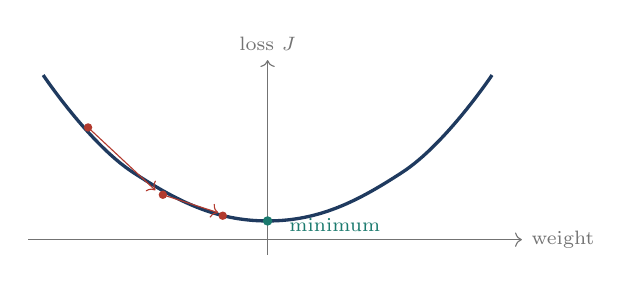
\begin{tikzpicture}[scale=0.95]
  \draw[->,black!55] (-3.2,0)--(3.4,0) node[right,font=\scriptsize]{weight};
  \draw[->,black!55] (0,-0.2)--(0,2.4) node[above,font=\scriptsize]{loss $J$};
  \draw[very thick,ink] plot[smooth,tension=0.7] coordinates{(-3,2.2)(-1.8,0.9)(0,0.25)(1.8,0.9)(3,2.2)};
  \fill[red] (-2.4,1.5) circle (1.6pt); \fill[red] (-1.4,0.6) circle (1.6pt);
  \fill[red] (-0.6,0.32) circle (1.6pt); \fill[grn] (0,0.25) circle (1.8pt);
  \draw[->,red] (-2.4,1.5)--(-1.5,0.66); \draw[->,red] (-1.4,0.6)--(-0.66,0.36);
  \node[grn,font=\scriptsize] at (0.9,0.2){minimum};
\end{tikzpicture}
\end{center}

\begin{intuition}
Read Equation~\eqref{eq:learnrule} in plain words: the correction to each weight is
\emph{(what the model predicted minus the truth) times the feature}. Predicted too
little hazard on a rough feature? $H-y$ is negative, so the rule pushes that weight up.
Too much? It pushes down. The model learns by repeatedly nudging weights in the
direction that would have made its past mistakes smaller. Every neural network on
Earth, however deep, is trained by versions of this one sentence.
\end{intuition}

\begin{example}[one learning step, by hand]
One sample, $\boldsymbol\zeta=(2,0)$, truth $y=1$, current weights $\mathbf w=(0,0)$,
$b=0$. Then $a=0$, $H=\sigma(0)=0.5$. The error is $H-y=-0.5$. The weight gradient is
$(-0.5)\cdot(2,0)=(-1,0)$. Stepping with $\eta=0.1$: $\mathbf w\leftarrow(0,0)-0.1\cdot
(-1,0)=(0.1,0)$. The first weight rose --- the model nudged itself toward calling this
rough sample hazardous. Repeat over many samples and the weights settle.
\end{example}

\begin{hatibox}
\textsc{Hati} skips this loop on purpose, but the door is open: feed it labelled safe
and hazardous sites and the same rule \eqref{eq:learnrule} would tune the ten weights.
The reason \textsc{Hati} does not is strategic --- fixed, physics-based weights need no
training data (which barely exists for lunar hazards) and stay interpretable and
certifiable. Knowing how learning \emph{would} work is what lets you make that choice
deliberately.
\end{hatibox}

\begin{practice}
\textbf{12.1} A sample has $\boldsymbol\zeta=(1,-1)$, $y=0$, and the model currently
outputs $H=0.7$. Find the error $H-y$ and the weight gradient $(H-y)\boldsymbol\zeta$.
Which weight goes up, which down, after a descent step? \quad\textbf{12.2} Why do we
take the log of the probabilities before summing, rather than multiplying them
directly? (Think about $0.01\times0.01\times\cdots$.)
\end{practice}

\section*{The rest of machine learning, in a paragraph}
Three ideas finish the toolkit, and you now have the footing for all of them.
\emph{Convexity:} for this loss the landscape is a single bowl (no false valleys), so
descent always finds the true bottom --- provable from the second derivative (the
\emph{Hessian}) being positive. \emph{Regularization:} add a penalty
$\tfrac{\lambda}{2}\norm{\mathbf w}^2$ to keep weights modest and avoid memorising
noise. \emph{Backpropagation:} in a deep network, the same ``error $\times$ input''
rule is applied layer by layer, the error carried backward by the chain rule using the
fact that $\sigma'(a)=\sigma(a)(1-\sigma(a))$. That is the whole of how modern networks
train; everything else is engineering.

% =====================================================================
\chapter{Why HATI is readable}

A deep network gives an answer and no reason. \textsc{Hati}'s single neuron gives both,
and the maths of why is short. Because the score before the sigmoid is a plain sum,
\begin{equation}
a=b+\sum_{k=1}^{10}\phi_k,\qquad \phi_k=\frac{w_k\zeta_k}{\norm{\mathbf w}_1},
\end{equation}
each channel's \emph{contribution} $\phi_k$ is a separate, addable number. So ``why did
this pixel score high?'' has an exact answer: list the $\phi_k$ and see which were big.
At the Athena touchdown, the slope-variation and small-crater-scale channels had large
positive $\phi_k$, while the average-tilt channels were near zero --- the texture, not
the steepness, raised the alarm.

\begin{keyidea}
When the inside is a sum, attribution is exact and free: the whole equals the sum of
its parts, so you can always say how much each part contributed. This is the deep
reason \textsc{Hati} is auditable where a black-box model is not --- and auditability
is what a mission needs before it trusts a number.
\end{keyidea}

\begin{practice}
\textbf{14.1} Two channels have weights $w=(1,0.6)$ (so $\norm{\mathbf w}_1=1.6$) and
standardised values $\zeta=(3,-1)$. Find each contribution $\phi_k$ and say which
channel drove the score and in which direction.
\end{practice}

% #####################################################################
\part{Geometry and signals}

% =====================================================================
\chapter{Matrices, eigenvectors, and the shadow ellipse}

\section{A matrix is a table that transforms vectors}
A \emph{matrix} is a rectangle of numbers. The only fact we need: a $2\times2$ matrix
can stretch and rotate vectors. For special vectors --- the \emph{eigenvectors} --- it
only stretches, not rotates; the stretch factor is the \emph{eigenvalue}. The
eigenvectors are the natural axes of whatever the matrix describes.

\section{Covariance: the shape of a cloud of points}
Take the pixels of a shadow blob. Their spread has a shape --- long one way, narrow the
other. The \emph{covariance matrix} captures it: the diagonal entries are how much the
points spread east--west and north--south, the off-diagonal how much the two go
together. Its eigenvectors point along the blob's long and short axes; its eigenvalues
are the squared lengths.
\begin{equation}
\mathbf M=\begin{pmatrix}\mu_{20}&\mu_{11}\\ \mu_{11}&\mu_{02}\end{pmatrix},\qquad
\lambda_{1,2}=\frac{\mu_{20}+\mu_{02}}{2}\pm\sqrt{\Big(\tfrac{\mu_{20}-\mu_{02}}{2}\Big)^2+\mu_{11}^2}.
\end{equation}

\begin{center}
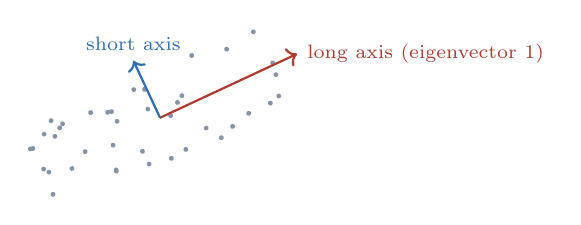
\begin{tikzpicture}[scale=0.8]
  \begin{scope}[rotate=25]
  \foreach \i in {1,...,40}{\pgfmathsetmacro{\px}{2.2*rand}\pgfmathsetmacro{\py}{0.7*rand}
     \fill[ink!55] (\px,\py) circle (1.1pt);}
  \draw[->,red,thick] (0,0)--(2.4,0) node[right,font=\scriptsize]{long axis (eigenvector 1)};
  \draw[->,blu,thick] (0,0)--(0,1.0) node[above,font=\scriptsize]{short axis};
  \end{scope}
\end{tikzpicture}
\end{center}

\begin{hatibox}
\textsc{Hati}'s shadow census fits an ellipse to each dark blob with exactly this
eigenvalue computation. The long axis (along the Sun) gives the shadow length $L$,
hence the obstacle height via $h=L\tan e$ from Chapter~2; the short axis gives the
footprint. The same algebra a statistician uses to find the axes of a data cloud finds
the dimensions of a shadow.
\end{hatibox}

\begin{practice}
\textbf{15.1} A diagonal covariance $\mathbf M=\big(\begin{smallmatrix}9&0\\0&1
\end{smallmatrix}\big)$ has eigenvalues $9$ and $1$ along the axes. Which way is the
blob long, and by what ratio of lengths (recall length $\propto\sqrt{\lambda}$)?
\end{practice}

% =====================================================================
\chapter{Mapping a sphere onto a sheet}

The Moon is a ball; our map is flat. The bridge is the \emph{stereographic projection},
and it comes from one picture and similar triangles.

Stand at the north pole $N$. For any surface point $P$, draw the straight line from $N$
through $P$ and continue it until it strikes the flat sheet laid against the south pole.
Where it strikes is where $P$ goes on the map. Two similar triangles in the slice
through $N$, $P$, and the pole give the map distance from the centre as
\begin{equation}
\rho=2R\tan\!\Big(\tfrac{\theta}{2}\Big),
\end{equation}
where $R$ is the Moon's radius and $\theta$ the angle of $P$ from the south pole.
Writing $\theta$ in terms of latitude $\varphi$ and adding the longitude $\lambda$ for
direction gives the working formula
\begin{equation}
\rho=2R\tan\!\Big(\tfrac{\pi}{4}+\tfrac{\varphi}{2}\Big),\qquad
X=\rho\sin\lambda,\quad Y=\rho\cos\lambda.
\end{equation}

\begin{intuition}
Shine every south-polar point up to the north pole and catch its shadow on a sheet
under the Moon. Near the south pole this barely distorts anything --- a metre on the
map is a metre on the Moon --- which is exactly the regime a polar landing cares about.
\end{intuition}

\begin{hatibox}
This is how \textsc{Hati} turns the published touchdown latitude and longitude into a
specific row and column on the elevation grid, so it can read the hazard score at the
exact spot the lander came down. Geometry, not guesswork, places the pixel.
\end{hatibox}

\begin{practice}
\textbf{16.1} At the south pole $\varphi=-90^\circ$. Show $\rho=0$, i.e.\ the pole maps
to the centre. (Use $\tan(\tfrac{\pi}{4}+\tfrac{\varphi}{2})$ with $\varphi=-\tfrac{\pi}{2}$.)
\end{practice}

% =====================================================================
\chapter{Sampling and the resolution floor}

Why is a \SI{4}{m} map ``blind below \SI{8}{m}''? Because of how sampling works --- the
same reason a low-quality audio recording loses the high notes.

When you record a signal by taking a value every $s$ metres (or every fraction of a
second), you can only faithfully capture wiggles slower than \emph{two samples per
wiggle}. Anything finer --- a bump that rises and falls within a single pixel --- cannot
be distinguished from something smoother; it ``folds'' into a false, slower shape. This
is the \emph{Nyquist--Shannon sampling theorem}, and the shortest wavelength you can
trust is twice the sample spacing:
\begin{equation}
\lambda_{\min}=2s.
\end{equation}

\begin{center}
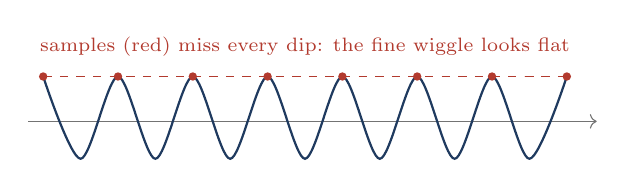
\begin{tikzpicture}[scale=0.95]
  \draw[->,black!55] (-0.2,0)--(7.4,0);
  \draw[thick,ink] plot[smooth,tension=0.5] coordinates{
    (0,0.6)(0.5,-0.5)(1,0.6)(1.5,-0.5)(2,0.6)(2.5,-0.5)(3,0.6)(3.5,-0.5)(4,0.6)(4.5,-0.5)(5,0.6)(5.5,-0.5)(6,0.6)(6.5,-0.5)(7,0.6)};
  \foreach \x in {0,1,...,7}{\fill[red] (\x,0.6) circle (1.6pt);}
  \draw[dashed,red] plot[smooth] coordinates{(0,0.6)(3.5,0.6)(7,0.6)};
  \node[font=\scriptsize,red] at (3.5,1.0){samples (red) miss every dip: the fine wiggle looks flat};
\end{tikzpicture}
\end{center}

For \textsc{Hati}'s $s=\SI{4}{m}$ elevation map, $\lambda_{\min}=\SI{8}{m}$: craters and
rocks smaller than that simply are not in the data. They are not faint --- they are
absent.

\begin{hatibox}
This floor is the entire reason \textsc{Hati} has a second channel. The shadow census
runs on a \SI{0.9}{m} photograph, whose floor is far lower, so it sees the
sub-\SI{8}{m} hazards the elevation map physically cannot. The two channels are not
redundant; they cover different size bands by design.
\end{hatibox}

\begin{practice}
\textbf{17.1} A different DEM has \SI{1.5}{m} pixels. What is its resolution floor?
\quad\textbf{17.2} In one sentence, why can a shadow in a \SI{0.9}{m} photo reveal a
\SI{2}{m} rock that a \SI{4}{m} elevation map cannot?
\end{practice}

% #####################################################################
\part{The summit}

% =====================================================================
\chapter{Reading the master equation}

You now own every piece. Let us read the wall, left to right, the way you would read a
sentence.
\begin{equation*}
H(x)=\sigma\!\left(b+\frac{1}{\norm{\mathbf w}_1}\sum_{k=1}^{10} w_k\,
\operatorname{clip}_{\pm c}\!\left[\frac{g(C_k[z])(x)-\operatorname{med}\,g(C_k[z])}{\operatorname{IQR}\,g(C_k[z])/1.349}\right]\right).
\end{equation*}

\begin{itemize}[leftmargin=1.5em]
\item $z$ is the elevation grid; $C_k[z]$ are the ten roughness fields, each a
\textbf{convolution / windowed statistic} (Chapters 6--7) of slope and curvature
(Chapters 4--5) computed from the grid.
\item $g=\log(1+\cdot)$ \textbf{tames the tail} (Chapter 1); subtracting the median and
dividing by $\operatorname{IQR}/1.349$ is the \textbf{robust $z$-score} (Chapters 8--9)
that puts all ten channels on one ruler; $\operatorname{clip}_{\pm c}$ caps outliers.
\item $\sum_k w_k(\cdots)$ is the \textbf{weighted sum / dot product} (Chapters 1, 3):
each standardised channel times its importance, added. Dividing by
$\norm{\mathbf w}_1$ keeps the scale steady.
\item $b$ is the bias; $\sigma(\cdots)$ is the \textbf{logistic squash} (Chapter 1)
that turns the score into a hazard probability $H(x)\in(0,1)$ --- the \textbf{logistic
neuron} of Chapter 11, with weights set from physics rather than learned (Chapter 12),
and \textbf{exactly attributable} channel by channel (Chapter 14).
\end{itemize}

\begin{keyidea}
Read aloud: ``Take the elevation grid; measure ten flavours of roughness; put each on a
common, outlier-resistant scale; add them up with physics-given importances; squash the
total into a probability.'' That sentence is \textsc{Hati}. You can now say it, and
defend every word.
\end{keyidea}

Alongside it runs Channel~2: detect shadows in the fine photograph, fit each an ellipse
by the covariance eigenvalues (Chapter 15), read its length and footprint, convert
length to height with $h=L\tan e$ (Chapter 2), and so census the obstacles that live
below the elevation map's \SI{8}{m} floor (Chapter 17). The stereographic projection
(Chapter 16) pins both channels to the right pixel.

\section*{So how do you become an expert?}
Understanding is the door; expertise is the room. Three steps through it.
First, do every \textsc{Practice} box with a pen --- the maths becomes yours only when
your own hand makes it. Second, read \texttt{hati\_math.pdf} again: the formal document
that this book was the key to; it will now read as plain prose. Third, change something
--- recompute a channel, alter a weight, run the pipeline on a new patch, and predict
the effect before you look. The moment you can predict what the equation will do before
the computer tells you, you are no longer learning the topic. You are doing it.

\appendix
\addcontentsline{toc}{part}{Appendices}

\chapter{Notation at a glance}
\begin{tabbing}
\hspace{3.2cm}\=\kill
$z,\ z_{ij}$ \> elevation grid and the height at row $i$, column $j$ \\
$s$ \> pixel size in metres (the ground sample distance) \\
$\nabla z$ \> gradient: the steepest-uphill arrow; its length is the slope \\
$\nabla^2 z$ \> Laplacian: curvature; $+$ in a pit, $-$ on a peak \\
$C_k[z]$ \> the $k$-th roughness channel (a convolution / windowed statistic) \\
$g(x)=\log(1+x)$ \> the tail-taming log \\
$\operatorname{med},\ \operatorname{IQR}$ \> median and interquartile range (robust spread) \\
$\zeta_k$ \> the $k$-th channel after standardising (a $z$-score) \\
$\mathbf w,\ b$ \> the weight vector and bias \\
$\norm{\mathbf w}_1=\sum_k\abs{w_k}$ \> the $\ell_1$ norm (sum of weight sizes) \\
$\sigma(a)=1/(1+e^{-a})$ \> the logistic / sigmoid \\
$H(x)$ \> the hazard probability at spot $x$, between $0$ and $1$ \\
$h=L\tan e$ \> obstacle height from shadow length $L$ and Sun elevation $e$ \\
$\lambda_{\min}=2s$ \> the resolution floor (Nyquist) \\
$\phi_k=w_k\zeta_k/\norm{\mathbf w}_1$ \> channel $k$'s contribution to the score
\end{tabbing}

\chapter{Solutions to the practice boxes}
\small
\textbf{1.1} $\sigma(0)=\tfrac12$; $\sigma(2)$ is closer to $1$ ($a>0$).\quad
\textbf{1.2} $a=2(1.5)-1(1)-1=1$; $\sigma(1)\approx0.73$.\quad
\textbf{1.3} $\log 0=-\infty$, undefined for a zero-valued channel; $\log(1+0)=0$ is fine.\\
\textbf{2.1} $h=6\tan20^\circ\approx\SI{2.2}{m}$.\quad
\textbf{2.2} $L=h/\tan5^\circ\approx 2.2/0.0875\approx\SI{25}{m}$; a low Sun reveals small hazards.\\
\textbf{3.1} $1(2)+0.7(-1)+0.7(3)=2-0.7+2.1=3.4$.\quad
\textbf{3.2} No --- positive weights mean a larger input only raises the sum; one rough channel can only push the hazard vote up.\\
\textbf{4.1} $f'(x)=6x$.\quad
\textbf{4.2} $\arctan(0.1)\approx5.7^\circ$; with both $0.1$, $\norm{\nabla z}=\sqrt{0.02}\approx0.141$, angle $\approx8.0^\circ$ --- steeper, because the two slopes combine by Pythagoras.\\
\textbf{5.1} $f''(x)=2>0$: a bowl.\quad
\textbf{5.2} Curvature is positive on the floor, negative at the rims.\\
\textbf{6.1} $4+4-2(9)=-10<0$: a peak (the recipe is the Laplacian; a bump gives negative).\quad
\textbf{6.2} It blurs (replaces each pixel by the average of its $3\times3$ neighbourhood).\\
\textbf{7.1} mean $=9.6$, median $=2$; the median is typical, the mean is dragged by $40$.\quad
\textbf{7.2} $Q_{25}=2.5$, $Q_{75}=6.5$, $\operatorname{IQR}=4$.\\
\textbf{8.1} $\hat s=2.698/1.349=2$.\quad
\textbf{8.2} median moves from $3$ to $3.5$ (barely); mean jumps from $3$ to $169.2$ --- the median is robust.\\
\textbf{9.1} $\zeta=(3-1)/(1.349/1.349)=2$.\quad
\textbf{9.2} $19/19$ below it among the others $\Rightarrow$ the top, the $100$th (or, of all $20$, the $95$th) percentile.\\
\textbf{10.1} $y=1\!:0.8$; $y=0\!:0.2$; more confident about hazard.\\
\textbf{11.1} $(2,0)\!:a=1,H\approx0.73$ (hazard); $(-2,0)\!:a=-3,H\approx0.05$ (safe).\\
\textbf{12.1} error $0.7$; gradient $0.7(1,-1)=(0.7,-0.7)$; after $-\eta\,$grad, $w_1$ down, $w_2$ up.\quad
\textbf{12.2} multiplying many small probabilities underflows to $0$; logs turn the product into a stable sum.\\
\textbf{14.1} $\phi_1=1\cdot3/1.6=1.875$, $\phi_2=0.6\cdot(-1)/1.6=-0.375$; channel 1 drove it strongly upward.\\
\textbf{15.1} long along the eigenvalue-$9$ axis; length ratio $\sqrt9:\sqrt1=3:1$.\\
\textbf{16.1} $\tan(\tfrac{\pi}{4}-\tfrac{\pi}{4})=\tan0=0\Rightarrow\rho=0$.\\
\textbf{17.1} $2\times1.5=\SI{3}{m}$.\quad
\textbf{17.2} the rock's shadow spans several \SI{0.9}{m} pixels even though the rock is smaller than one \SI{4}{m} elevation pixel.

\chapter{Where to go next}
\begin{itemize}[leftmargin=1.4em]
\item \texttt{hati\_math.pdf} --- the rigorous companion this book unlocks.
\item Calculus and linear algebra: any first-year university text, or the free
\emph{3Blue1Brown} ``Essence of'' video series for the pictures behind Chapters 4--5
and 15.
\item Machine learning: the logistic-regression chapter of any introductory course
gives Chapters 11--13 in full.
\item Lunar terrain: Kreslavsky \& Head (2000) and Rosenburg et al.\ (2011) for the
roughness operators; Hapke (1984) for the shadow photometry; Henriksen et al.\ (2017)
for how the elevation maps are made.
\end{itemize}

\end{document}
